%%
%
% Gnikwo
% gnikwo@hotmail.com
%
%%

\documentclass[a4paper]{report}

%packages
\usepackage[utf8]{inputenc}
\usepackage[francais]{babel}
\usepackage{graphicx}\graphicspath{{pix/}}
\usepackage{float}
\usepackage[T1]{fontenc}
\usepackage{color}
\usepackage{fancyhdr}
%Options: Sonny, Lenny, Glenn, Conny, Rejne, Bjarne, Bjornstrup
\usepackage[Bjornstrup]{fncychap}
\usepackage[procnames]{listings}
\usepackage[colorlinks=true,linkcolor=black]{hyperref}
\usepackage{pdfpages}
\usepackage{titlesec, blindtext, color}

%pdf metadata
\hypersetup{
    unicode=true,
    colorlinks=true,
    citecolor=black,
    filecolor=black,
    linkcolor=black,
    urlcolor=black,
    pdfauthor={Nicolas Ballet <gnikwo@hotmail.com>},
    pdftitle={},
    pdfcreator={pdftex},
    pdfsubject={},
    pdfkeywords={},
}


\definecolor{keywords}{RGB}{200,0,90}
\definecolor{comments}{RGB}{0,0,113}
\definecolor{red}{RGB}{160,0,0}
\definecolor{green}{RGB}{0,150,0}

%inner meta
\title{Rapport LO43}
\author{Nicolas Ballet, Nicolas Vincent, Marine Collet, Lucas Demouy}
\date{\today}


\begin{document}

\maketitle

\tableofcontents

\chapter{Background}

\section{Attentes}

Le but de ce projet était de montrer que nous avons appris à créer un programme ayant une structure générique et
réutilisable dans le cadre de l'UV LO43.

\section{Choix du sujet}

Nous étions intéressés par l'un des sujets proposés par M.Creput: "Développement d'un framework permettant de créer et de
gérer des interfaces graphiques". Initialement, ce sujet propose donc de concevoir et de développer un framework en
Java permettant, lorsque nous avons une application déjà existante de pouvoir y greffer une interface graphique, et cela
de manière simple. On doit donc pouvoir définir des paramètres liés à l'application, ainsi que des boutons contrôlant
son fil d'exécution (Start / Stop / Pause / Pas à pas).
S'approprier son sujet étant très important, nous y avons apporté des
modifications. Nous sommes donc partis sur un développement en C++, utilisant OpenGL pour le rendu graphique, et
utilisant des threads afin de séparer l'interface graphique et le cœur de l'application. Le
framework doit pouvoir être compilé aussi bien sur Windows que sur un système Unix.

    \vspace{5mm}

Nos modifications impliquaient l'implémentation d'un moteur graphique. Mais cela faisait aussi appel à beaucoup de
généricité, nous nous sommes donc concentrés la dessus.

\section{Objectifs}

Finalement, notre sujet s'est formalisé comme ceci :
Création d'un framework multi-os performant, permettant de créer des interfaces sur des applications pré-existantes ou
non. Il devra être capable d'être étendu simplement (l'utilisateur du framework doit pouvoir facilement créer de
nouveaux types d'éléments graphiques). Il devra aussi comporter une gestion des appuis clavier et des clics souris.


\chapter{Analyse}

    \section{Cas d'utilisations}

    Nous avons commencé par définir un diagramme de cas d'utilisations :
\begin{center}
    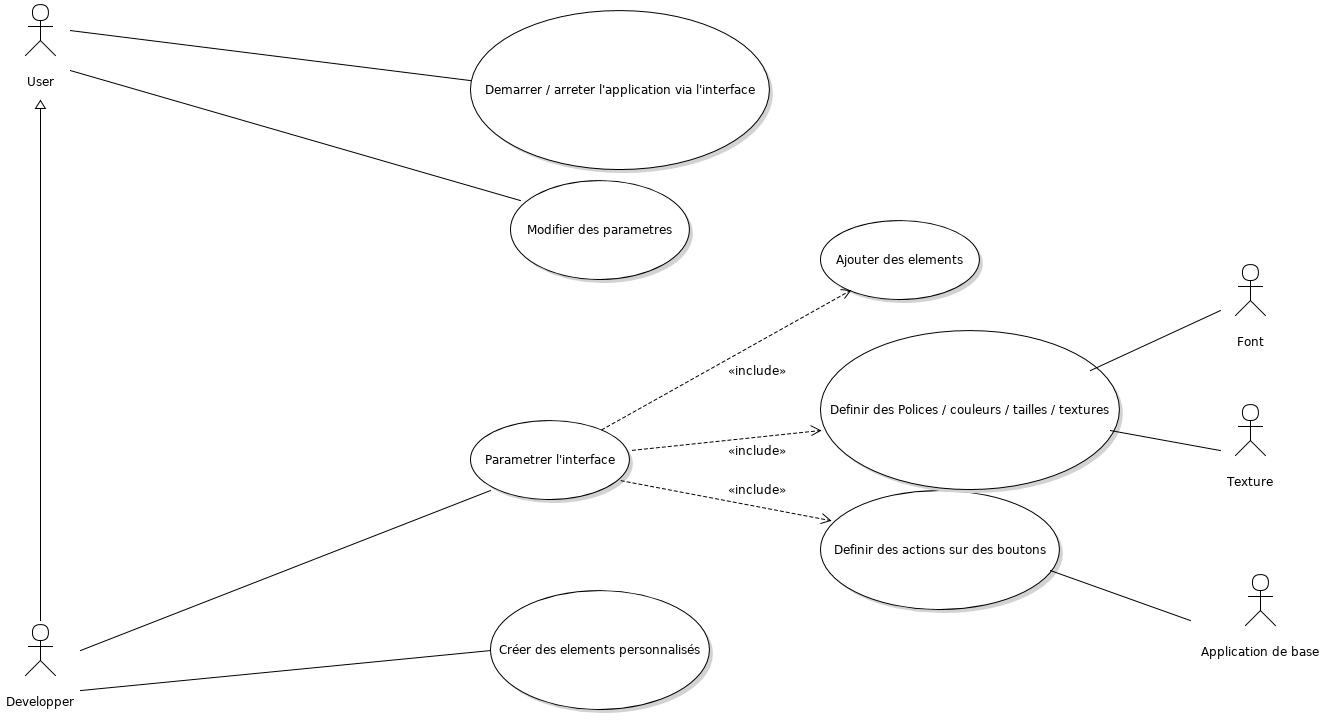
\includegraphics[scale=0.3]{Analyse/UseCase.png}
\end{center}

    \section{Classes}

    Nous avons ensuite défini le diagramme de classe :
\begin{center}
    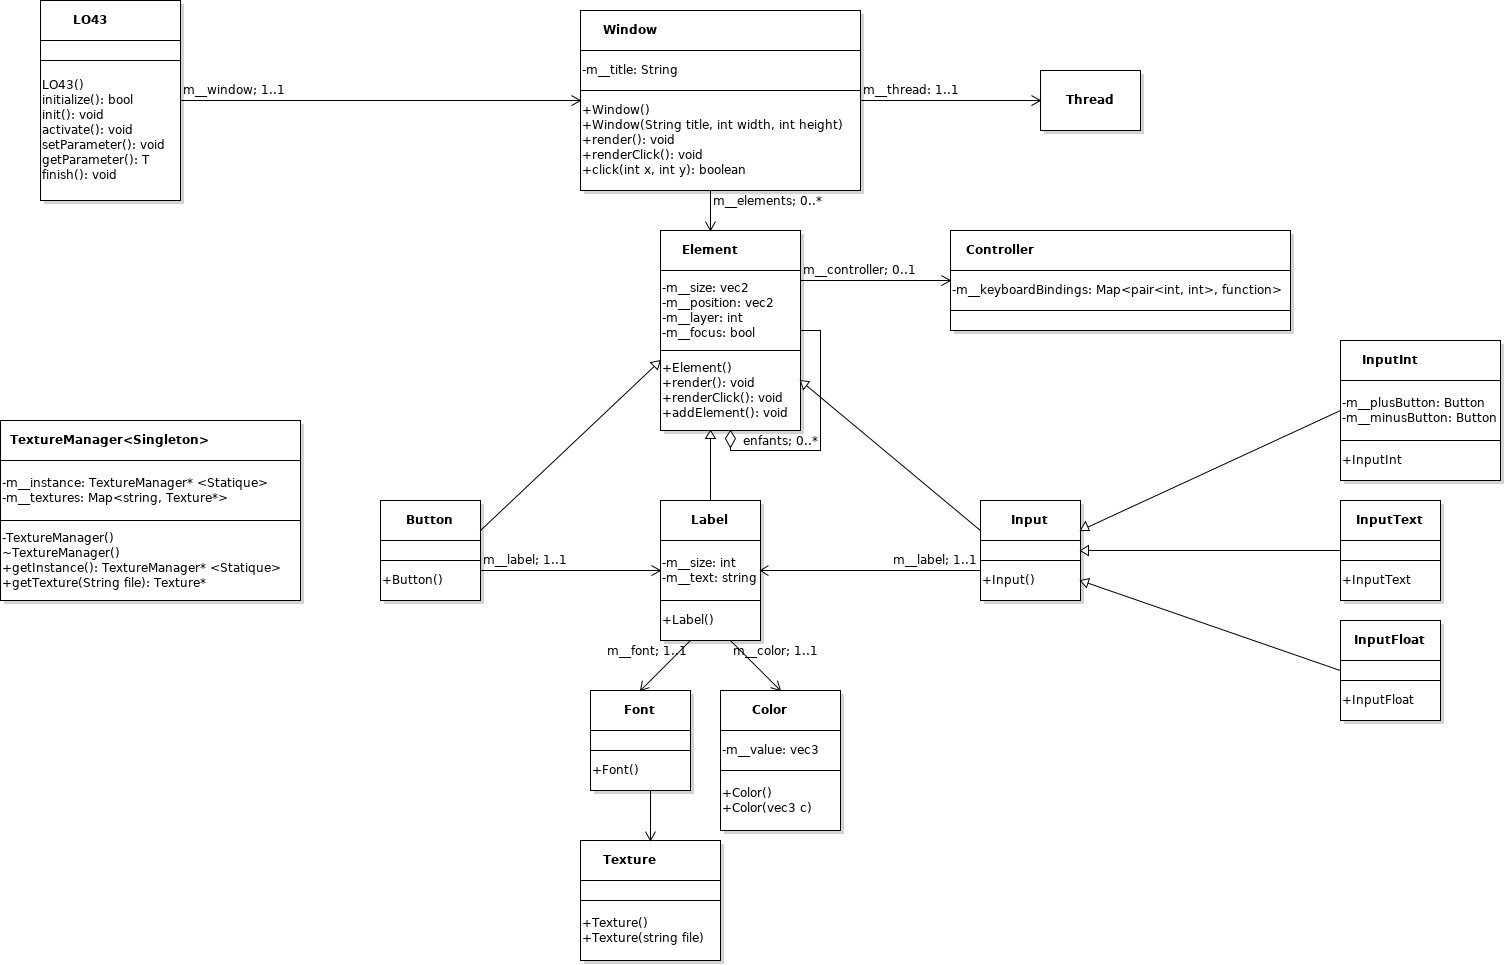
\includegraphics[scale=0.3]{Analyse/Classes.png}
\end{center}

    \section{Gestion de projet}

    Afin de nous organiser et de gérer notre projet, nous avons utilisé plusieurs outils :
\begin{itemize}
    \item git, git bash et github, pour simplifier la gestion du code source.
    \item CMake, pour ne pas avoir à compiler à la main en se souciant de l'OS.
    \item Violet UML Editor, pour tout ce qui concerne les diagrammes UML.
    \item Valgrind, Valgrind est un paquet linux permettant de suivre les allocations et de prévenir des fuites mémoires ou
    d'utilisation de variables non initialisées.
\end{itemize}

    \vspace{5mm}

    L'optique de notre projet étant d'être plus qu'un projet d'étude, nous l'avons placé sous licence LGPL.v3, qui
    permet la réutilisation libre et gratuite du code source.

\chapter{Fonctionnement}

    Les exemples présents dans ce chapitre se baseront sur cette fenêtre :
\begin{center}
    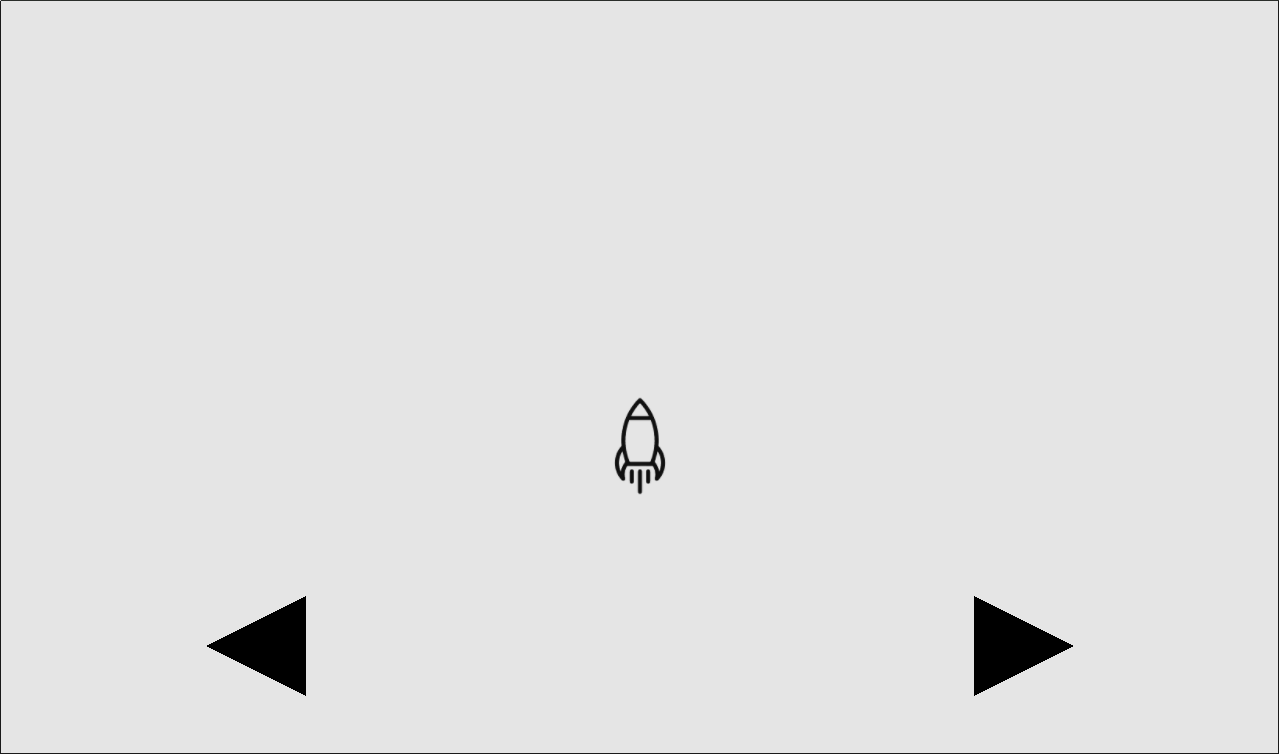
\includegraphics[scale=0.3]{Analyse/Capture.png}
\end{center}

    \section{Initialisation}

    Le déroulement normal de l'execution se découpe en sous partie, et pour commencer il y a tout d'abord une phase d'initialisation.
    C'est durant cette phase que la fenêtre et le context OpenGL sont crées.
    Les dictionnaires de fenetres, textures et d'objets, shaders sont initialisés.

    \vspace{5mm}

    Ces dictionnaires font en sorte de ne pas importer deux fois la même texture, fenetre, \ldots.

    \vspace{5mm}

    Les éléments graphiques sont créés et l'ensemble des points qui définissent leurs formes sont envoyés à la carte
    graphique.

    \vspace{5mm}

    Les textures sont aussi chargées et envoyées à la carte graphique.

    \vspace{5mm}

    Les shaders, sont des programmes utilisés par la carte graphique afin de rendre une image. C'est pendant la phase
    d'initialisation qu'ils sont compilés et envoyés à la carte graphique.

    \vspace{5mm}

    Le lien entre appui clavier et action sont définis. C'est ici que le lien avec l'application métier est effectué.

    \vspace{5mm}

    Et enfin, l'arbre des objets et construit.

    \vspace{5mm}

    L'arbre des objets représente la hiérarchie des objets affichés dans la fenêtre.

    \section{Boucle de rendu}

    La boucle de rendu est découpée en plusieurs parties :
\begin{itemize}
    \item Vérification des appuis claviers
    \item Vérification des clics souris
    \item Rendu des éléments graphiques
\end{itemize}

    \vspace{5mm}

    La vérification des appuis claviers se fait simplement avec des fonctions lambda, si une touche est enfoncée puis
    relachée, on exécute la fonction associée.

    \vspace{5mm}

    Tandis que la vérification des clics souris est un peu plus longue. Notre objectif ici était de gérer des éléments de
    forme complexe. L'algorithme AABB ne remplissait pas cette condition, nous avons donc opté pour un système de lancé
    de rayon.

    \vspace{5mm}
    Chaque élément se voit attribuer une couleur unique lors de sa création. Cette couleur est utilisée lors du lancer de
    rayon :

\begin{center}
    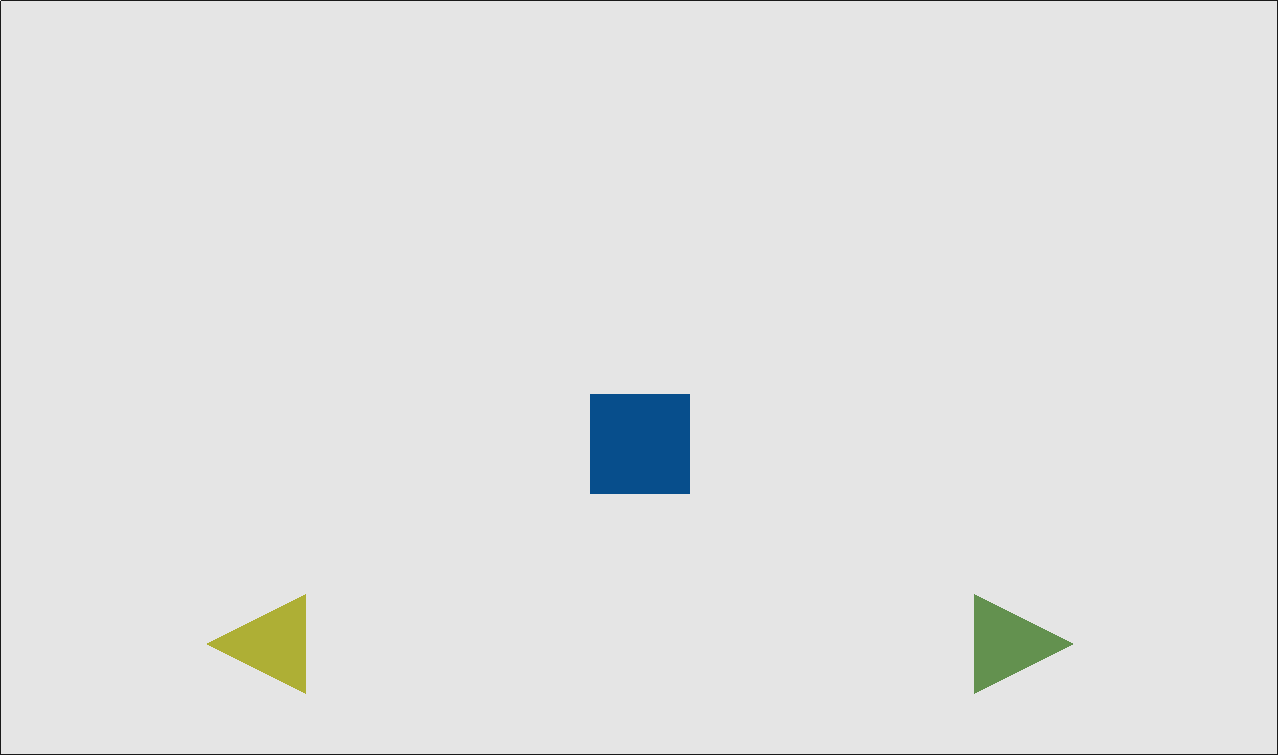
\includegraphics[scale=0.3]{Analyse/Click.png}
\end{center}

    Il ne reste plus qu'à récupérer la couleur se trouvant sous la souris et de récupérer l'élément associé à celle-ci.

    \vspace{5mm}

    Le rendu final de la fenêtre est enfin effectué en parcourant l'arbre en profondeur.

    \section{Fermeture}

    La boucle de rendu se termine lorsque l'on veut fermer la fenêtre.

    \vspace{5mm}

    C'est donc au tour de la désallocation d'entrer en scène.
    Les dictionnaires de Texture, etc, sont vidés en libérant les objets contenus.
    La fenêtre, le contexte OpenGL ainsi que la mémoire graphique sont liberés.

    \vspace{5mm}

    Et le programme se termine.

\chapter{Un peu plus en détails}

    \section{Dictionnaires de données}

        Afin de ne pas avoir de redondance d'informations, nous avons mis en place un dictionnaire de données basé sur
        des templates.

        Nous avions prévu de d'implémenter un manager de données afin de gérer automatiquement l'importation d'une
        ressource non présente dans le dictionnaire. Mais un manque de temps nous a forcé a abandonner l'idée.

        Nous aurions voulu ici utiliser des "std::shared\_ptr" afin que la désallocation soit automatique, mais nous n'avions
        pas connaissance de cette classe au début du projet, et le temps ne nous a pas permis de faire évoluer la
        classe.

    \section{Controller}

        Une autre classe importante est la classe Controller. Si une autre classe hérite de Controller, alors il devient
        possible d'associer l'appui d'une touche clavier à une action sur cet objet.

    \vspace{5mm}

        Exemple :


    \begin{lstlisting}

            Button* b = (Button*) Gif::addElement("Test", new Button());

            b->load();

            b->bind(GLFW_KEY_A, [&b]() {

                b->action();

            });
    \end{lstlisting}


    \section{Element}

        La classe Element est certainement la plus importante, elle est la base de tous les éléments affichés à
        l'intérieur de la fenêtre.

    \vspace{5mm}

        Elle comporte l'allocation et le transfert des données vers la carte graphique, mais aussi le "draw call" qui
        est la demande à la carte graphique de générer un rendu via le shader, et les données actuellement utilisées.

    \vspace{5mm}

        Tout objet héritant de Element va pouvoir définir les points qui définissent sa forme, les données qui doivent
        être envoyées à la carte graphique lors du rendu, mais aussi un shader personnalisé si la méthode de rendu par
        défaut ne suffit pas, etc.

    \vspace{5mm}

        Exemple avec la classe Button :

    \begin{lstlisting}

        #Dans le constructeur:

        addPoint(vec3( 0.0, -1.0, 0.0));
        addPoint(vec3( 0.0,  0.0, 0.0));
        addPoint(vec3( 1.0, -1.0, 0.0));

        addPoint(vec3( 0.0,  0.0, 0.0));
        addPoint(vec3( 1,  0.0, 0.0));
        addPoint(vec3( 1.0, -1.0, 0.0));

        addIntUniform("pressed", &(m__pressed));

    \end{lstlisting}

    Une déclaration simple de deux triangles composant la classe Button,
    ainsi que la déclaration de la variable m\_\_pressed qui sera envoyée au shader sous le nom "pressed".

    \section{Thread}

        Afin de rester multi-plateforme, nous avons créé une classe Thread pouvant être compilée sous Unix et sous
        Windows, cela via un jeu d'inclusion et un simple test lors de la compilation. Mais du point de vue du code
        source, il n'y a qu'une classe Thread. Nous avons suivi le même procédé pour la gestion des mutex.

\chapter{A posteriori}

    \section{Problemes rencontrés}

    Nous avons utilisé CMake afin de générer automatiquement des Makefile sous Unix et sous Windows, malheureusement
    son comportement diffère sur les deux systèmes. Le code est donc compilable à la main sur Windows mais pas via CMake, ce qui à
    été un gros handicap durant le développement.

    \vspace{5mm}

    Le manque de temps a aussi été un vrai problème. Ou plutôt, (pour voir le problème dans l'autre sens) nous avons vu
	beaucoup trop grand et avons mal estimé le temps de travail.

    \vspace{5mm}

    Nous avons aussi rencontré des problèmes de fuite mémoire, mais nous les avons corrigés assez vite via Valgrind.

    \section{Conclusion}

    Finalement, le projet est utilisable, mais tous les objectifs que nous nous avions fixés au départ n'ont pas été
    atteints. Les threads sont implémentés mais ils ne sont pas utilisés. Le projet n'est pas complètement multi-os
    étant donné qu'il faut le compiler à la main sous Windows.
    En mettant cela de côté, ce projet a vraiment été intéressant. La recherche de l'optimisation, de la simplicité
    d'utilisation et de la généricité était assez satisfaisante.

    \vspace{5mm}

    Nous allons continuer de développer ce projet afin de terminer le travail commencé. Le projet étant réellement
    utilisable, il serait dommage de le laisser dépérir.

\addtolength{\textheight}{60mm}


\end{document}

